\documentclass[twoside,11pt]{article}

\usepackage{jmlr2e}

\usepackage[utf8]{inputenc}
\usepackage{amsmath, latexsym}
\usepackage{tikz}
\usepackage{xcolor}
\usepackage{xspace}
\usepackage{wrapfig}
\usepackage{pdfpages} % for including full-size landscape pdf
\usepackage[printonlyused,withpage]{acronym}


\acrodef{YOLO}[YOLO]{You Only Look Once}
\acrodef{ALPR}[ALPR]{Automatic License Plate Recognition}
\acrodef{LPCS}[LPCS]{Licence Plate Character Segmentation}
\acrodef{LP}[LP]{Licence Plate}
\acrodef{NN}[NN]{Neural Network}
\acrodef{OCR}[OCR]{Optical Character Recognition}


\firstpageno{1}

\begin{document}

\title{
    Image Processing Group Project Proposal\\
    Automatic Number-Plate Recognition\\
    2022/23 Fall Semester
}

\author{\name Barnabás Börcsök
    \email barnabas.borcsok@edu.bme.hu
    \AND
    \name Gergő Haragos
    \email TODO
   \AND
    \name Zoltán Simon
    \email zoltan.simon@edu.bme.hu
   \AND
    \name Bence Sándor Szabó 
    \email TODO
   \\\vfill\hfill\addr Budapest University of Technology and Economics
}

\maketitle

\section{Introduction}
\section{Introduction}
\todo[inline]{Proofread + Actualize introduction section}

There are many use cases in traffic control, where the \ac{LP} of vehicles must
be read.  This task can be automated by computers. A wall-mounted or even
hand-held camera can take pictures of cars. The image then can be processed by
various algorithms to detect the \ac{LP}, segment the characters and finally
recognise these characters.  In recent years with the increasing amount of
traffic, the need for well-performing \ac{ALPR} systems has increased
substantially.

We propose our own \ac{ALPR} implementation.  We write about the
state-of-the-art literature of the field. Our solution will be based on some of
these publications. Our goal when selecting from the many available methods was
to select the methods with the most promising test results.

We provide a project outline describing our planned tasks. The development
process can be split up into a few large portions. This is visualised on a Gantt
chart, where you can review each subtask.

After successful implementation, we will test our work on predefined training
data as well as further real-life data. We also list some evaluation
considerations.

Our implementation at \url{https://github.com/bobarna/bme-image-processing},
with detailed, reproducable steps.

\todo[inline]{Add document outline here.}


\section{Previous Solutions}
\csection{Previous Solutions}
\label{previous-solutions}

\subsection{Automatic Number-Plate Recognition}
\label{previous-solutions-anpr}
% Section label
In the past years many research projects have been focused on \ac{ALPR}.
We have surveyed some of the most recent and most promising works in this field.
A recent survey by \cite{survOnMet} gives an overview of different methods and
practices used in \ac{ALPR}.

Texture-based methods use characters present on the \ac{LP} as the basis for
\ac{ALPR}. Significant color difference between the board and its characters
creates a high-frequency color transition. If the image is grayscale,
there is an easy to distinguish change of colors between the characters and the
background of the board. This creates a unique pixel intensity distribution in
the region of the plate. The plate region should have a high edge density. This
is used in edge-based systems. In \cite{HongFuJiaHuan} the authors used
scan-line technique for \ac{ALPR}.

Introduced by \cite{redmon2016look} as a novel object detection method,
\ac{YOLO} serves as the basis for the \ac{ALPR} introduced by
\cite{DBLP:journals/corr/abs-1909-01754}.
The naming of \ac{YOLO} comes from the fact that it performs the object detection
for the full image in a single pass. The employed \ac{NN} divides the image
into regions and predicts bounding boxes and probabilities for each region.
Building on this method the authors achieved a license plate recognition rate of
$96.9\%$.  The method was tested on multiple different datasets with outstanding
results.  Besides the novel approach, the authors of this work also released
a public dataset of $38,351$ manually labeled bounding boxes on $6,239$ images.

A benchmark for \ac{ALPR} is introduced by
\cite{DBLP:journals/corr/GoncalvesSMS16}. This benchmark is
composed of a dataset helping the \ac{LPCS} step. High success rate of this step
is crucial for end-to-end success of \ac{ALPR}. Besides the dataset, the authors
also propose a new evaluation measure of the location of the bounding
box within the ground-truth annotation. To further optimise the \ac{LPCS} step,
they suggest a more straightforward approach to perform it efficiently.

\subsection{Optical Character Recognition}
\label{previous-solutions-ocr}
\todo[inline]{Write OCR previous solutions section (Zoli's excellent
notebook is a good starting point)}


\section{Proposed Method}
Outline our proposed method

TODO figure for training

TODO figure for the deployed solution

What kind of data are we going to use?


\section{Project Outline}
See figure~\ref{gantt}.


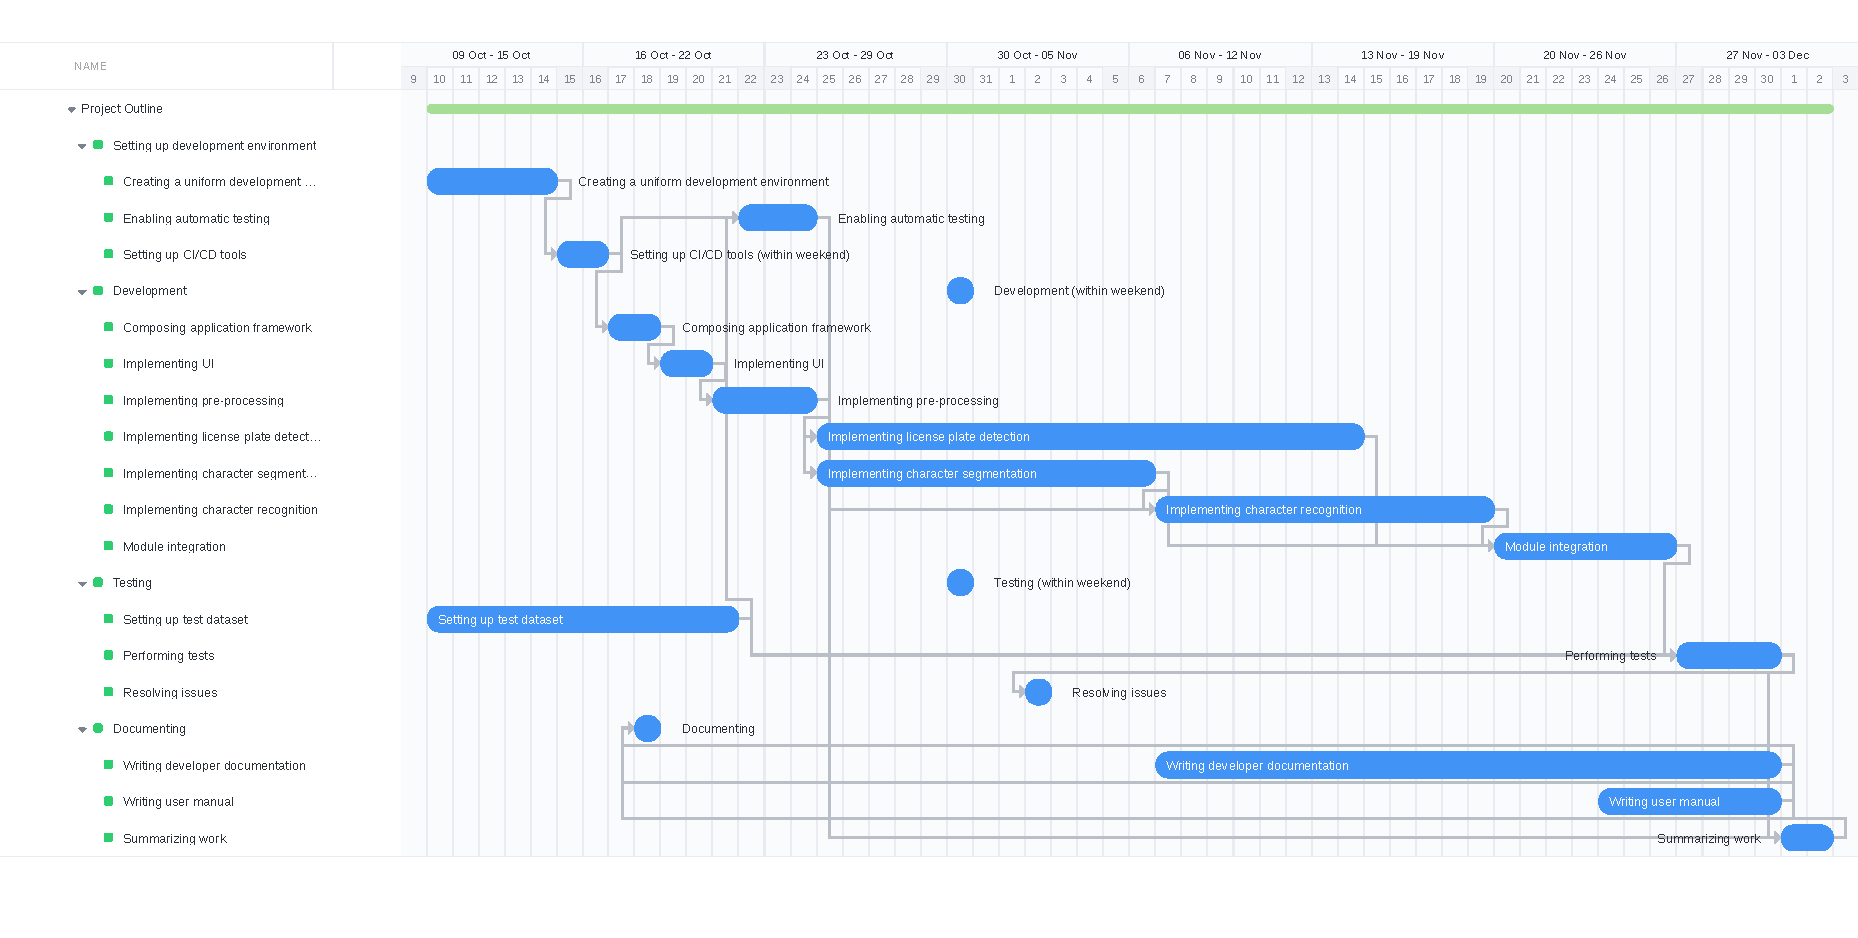
\includepdf[landscape=true,pages=-,addtotoc={
    1,section,1,Gantt Diagram, gantt
}]
{resources/gantt.pdf}


\section{Evaluation Method}
Propose the evaluation metrics, and the possibility of using real life data
later on.



\newpage
\bibliography{literature.bib}
\newpage


\end{document}
